% main.template.tex is the source of the paper. Do not edit main.tex by hand:
% `python -m pressure_probe.cli report --config <cfg>` renders main.tex from this file,
% filling the RES, RESTXT, RESTABLE and RESFIG tokens from results/<run>/summary.json.
% Any value that has no measured result renders as a yellow [todo].
\documentclass[conference]{IEEEtran}
\IEEEoverridecommandlockouts
\usepackage{cite}
\usepackage{amsmath,amssymb,amsfonts}
\usepackage{algorithmic}
\usepackage{graphicx}
\usepackage{textcomp}
\usepackage{xcolor}
\usepackage{booktabs}
\usepackage{multirow}
\usepackage{array}
\usepackage{adjustbox}
\usepackage{url}
\usepackage{tikz}
\usetikzlibrary{arrows.meta,positioning}

\newcommand{\TODO}{\colorbox{yellow}{[todo]}}
\newcommand{\REVIEW}[1]{\par\noindent\colorbox{yellow}{\parbox{\dimexpr\linewidth-2\fboxsep\relax}{\footnotesize\textbf{[todo: author review]} #1}}\par}
\newcommand{\cps}{\textsc{cps}}
\newcommand{\dfr}{\textsc{dfr}}

\begin{document}

\title{Consistent but Wrong: Detecting Repeated LLM Errors by Doubting the Answer}

\author{
\IEEEauthorblockN{\RES{author.1.name}}
\IEEEauthorblockA{\RES{author.1.affiliation}\\
\RES{author.1.email}}
\and
\IEEEauthorblockN{\RES{author.2.name}}
\IEEEauthorblockA{\RES{author.2.affiliation}\\
\RES{author.2.email}}
\and
\IEEEauthorblockN{\RES{author.3.name}}
\IEEEauthorblockA{\RES{author.3.affiliation}\\
\RES{author.3.email}}
}

\maketitle

\begin{abstract}
Detectors that sample a model several times flag a hallucination when the answers disagree. They miss the case in which the model gives the same wrong answer every time. These consistent errors do not shrink as models grow, and the one detector shown to catch them needs hidden states from two models and labelled training data. We ask whether a simple challenge separates consistent errors from consistent correct answers when only generated text is available. After answering, the model is asked in three phrasings whether it is sure, each in a separate conversation, and the doubt flip rate (\dfr{}) is the share of replies that abandon the answer. We also test a contrastive variant that subtracts the doubt flip rate from the flip rate under counterclaims naming a plausible alternative, which was meant to remove the general tendency to agree with the user. On a matched set of consistently wrong and consistently right answers from TruthfulQA, TriviaQA and SciQ for \RES{m1.name} and \RES{m2.name}, we compare \dfr{} with seven baselines, including Semantic Entropy, SelfCheckGPT and MetaQA, on identical items with paired tests. \RESTXT{abstract.results} \dfr{} needs \RES{set.dfr_calls} generations per question, no training, and no access to logits or weights.
\end{abstract}

\begin{IEEEkeywords}
hallucination detection, large language models, uncertainty estimation, consistency, sycophancy, black box evaluation
\end{IEEEkeywords}

\section{Introduction}

Large language models state false facts in fluent, confident prose. When their answers feed search results, retrieval pipelines or agents, an undetected error is passed on as fact. A widely used family of detectors works only from the text a model produces: the model answers the same question several times, and disagreement among the answers is read as a sign that it does not know~\cite{manakul2023selfcheckgpt,kuhn2023semantic,farquhar2024detecting,lin2024generating,nikitin2024kernel}. A model that knows the answer puts most of its probability on it, while a model that does not spreads probability over several plausible answers.

That reasoning fails when the model is wrong in the same way every time. Asked what share of the brain humans use, a model may answer ``about 10\%'' in every sample, and SelfCheckGPT then gives the myth a low hallucination score~\cite{yang2025metaqa}. Tan et al.~\cite{tan2025consistent} call such cases self-consistent errors. As models grow, inconsistent errors become rarer while consistent errors stay level or increase, and Semantic Entropy scores close to or below chance on them. Ganesh et al.~\cite{ganesh2026rethinking} reach a similar conclusion across 16 models, and studies of high certainty hallucinations find that a sizeable share of errors comes with high confidence~\cite{simhi2025trust,xu2025delusions}. The method of Tan et al. for these errors trains probes on the hidden states of the target model and of a second verifier model, so it cannot be applied to a model served only through an API.

We test a cheaper signal. Instead of asking the same question again, we doubt the answer. Models often change an answer when a user pushes back~\cite{sharma2023sycophancy,laban2023flipflop}, and they switch less often when the original answer was right~\cite{kim2025challenging,pawitan2025confidence}. We turn this into a training free detector: the doubt flip rate (\dfr{}) is the share of replies to ``Are you sure?'' style prompts that abandon the answer. We also test a contrastive variant (\cps{}) that subtracts the doubt flip rate from the flip rate under counterclaims naming an alternative. \cps{} was our original main score, designed to remove general agreeableness. A pilot study, whose items are excluded from every reported number, suggested that this subtraction removes the signal instead, so before the full run we made \dfr{} the main score, fixed new criteria and kept \cps{} as a hypothesis to test.

This paper makes four contributions.
\begin{enumerate}
\item We evaluate the doubt flip rate as a training free, text only detector of consistent errors, the case where sampling based detectors and certainty based abstention fail.
\item We build a matched evaluation set of consistently wrong and consistently right answers for two open models on three datasets and release every sampled answer and every reply to doubt.
\item We compare \dfr{} with seven baselines, including MetaQA, on identical items with paired statistical tests and report the cost of each method.
\item We test whether controlling for general agreeableness helps, by comparing \dfr{} with the contrastive score \cps{}, and whether a cheap check against another model family adds to \dfr{}.
\end{enumerate}
\RESTXT{intro.findings}

Section~\ref{sec:related} reviews related work, Section~\ref{sec:method} defines the scores, Section~\ref{sec:setup} describes the protocol, and Sections~\ref{sec:results} to~\ref{sec:limits} report and discuss the results.

\section{Related Work}\label{sec:related}

\textbf{Detection from consistency and confidence.} SelfCheckGPT compares an answer with sampled answers using NLI, question answering or n\,gram overlap~\cite{manakul2023selfcheckgpt}. Semantic Entropy groups sampled answers by bidirectional entailment and computes entropy over meanings~\cite{kuhn2023semantic,farquhar2024detecting}; Kernel Language Entropy and graph based measures change how the similarity between answers is used~\cite{nikitin2024kernel,lin2024generating}. Other detectors read the model's own confidence: token probabilities, the probability that the model calls its answer true~\cite{kadavath2022language}, or a confidence stated in words~\cite{xiong2024express}. Xue et al.~\cite{xue2026verify} show that adding a verifier model raises the ceiling of self consistency methods. SAC3 combines question perturbation with checks across models~\cite{zhang2023sac3}, Goel et al. use agreement across frontier models~\cite{goel2025zero}, and Semantic Reformulation Entropy paraphrases the question~\cite{tong2025sre}. All of these rely on disagreement somewhere, which a consistent error does not show.

\textbf{Consistent and high certainty errors.} Tan et al.~\cite{tan2025consistent} define self-consistent errors on TriviaQA and SciQ and propose a cross model probe on hidden states. Ganesh et al.~\cite{ganesh2026rethinking} find that consistent errors dominate TruthfulQA. Simhi et al.~\cite{simhi2025trust} show that 10 to 40 percent of hallucinations exceed a well chosen certainty threshold, and Xu et al.~\cite{xu2025delusions} call high belief errors delusions and find that models insist on them more than on ordinary hallucinations when asked to reflect. Zhou et al.~\cite{zhou2026confabulations} and Orgad et al.~\cite{orgad2025llms} show that confidence and correctness can come apart. None of these studies offers a black box, training free detector for this error type.

\textbf{Challenging the answer.} In the FlipFlop experiment, ``Are you sure?'' lowered accuracy across many models~\cite{laban2023flipflop}, and models trained with human feedback often agree with a user against the truth~\cite{sharma2023sycophancy}. Several studies note that answers change less often when they were right: Pawitan and Holmes find kept answers far more accurate than changed ones after ``think again''~\cite{pawitan2025confidence}, Kim and Khashabi find models switch less to a rebuttal when originally correct~\cite{kim2025challenging}, SycEval reports more corrections than reversals~\cite{fanous2025syceval}, and Guo et al. relate conformity to epistemic uncertainty~\cite{guo2026conformity}. Huang~\cite{huang2026sycophancy} shows that a flip rate mixes corrections with capitulations. Closest to our method, QueRE asks about 50 further questions about the answer, including ``Are you sure?'', reads the probabilities of their answers and trains a classifier on correctness labels~\cite{sam2025quere}. Our score needs no labels, no probabilities and no training, and we evaluate it on exactly the consistent errors that sampling misses.

\textbf{Perturbation and metamorphic testing.} MetaQA asks the model for synonym and antonym versions of its answer and scores how often these relations are violated~\cite{yang2025metaqa}. Counterfactual probing measures how the model's confidence moves between a statement and altered versions~\cite{feng2025counterfactual}, and Joo et al. study consistency under expressed uncertainty~\cite{joo2025uncertain}. MetaQA is the closest black box method, so we include it as a baseline.

\section{Method}\label{sec:method}

\begin{figure}[t]
\centering
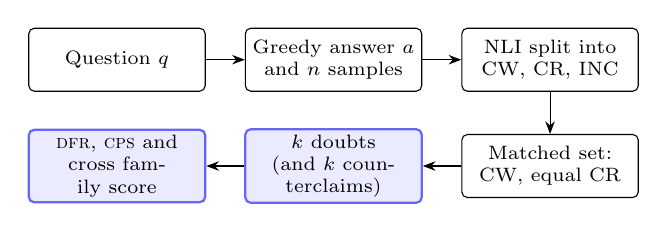
\begin{tikzpicture}[every node/.style={font=\scriptsize}, box/.style={draw, rounded corners=2pt, align=center, minimum height=8mm, text width=21mm, inner sep=2pt}, ours/.style={box, fill=blue!8, draw=blue!60, thick}, >={Stealth[length=1.6mm]}]
\node[box] (q) at (0,0) {Question $q$};
\node[box] (g) at (2.75,0) {Greedy answer $a$\\and $n$ samples};
\node[box] (s) at (5.5,0) {NLI split into\\CW, CR, INC};
\node[box] (m) at (5.5,-1.35) {Matched set:\\CW, equal CR};
\node[ours] (p) at (2.75,-1.35) {$k$ doubts\\(and $k$ counterclaims)};
\node[ours] (c) at (0,-1.35) {\dfr{}, \cps{} and\\cross family score};
\draw[->] (q) -- (g); \draw[->] (g) -- (s); \draw[->] (s) -- (m); \draw[->] (m) -- (p); \draw[->] (p) -- (c);
\end{tikzpicture}
\caption{Evaluation pipeline. All baselines reuse the sampled answers of the second step; only the challenges (shaded) add generations, and only for consistent answers.}
\label{fig:pipeline}
\end{figure}

\subsection{Problem setup}

Let $M$ be a model and $q$ a question with reference answers. The greedy answer $a=M(q)$ is decoded at temperature 0, and $n$ further answers $s_1,\dots,s_n$ are sampled at temperature $T$. Two answers $x$ and $y$ are equivalent, $E(x,y)=1$, when an NLI model judges that ``$q$~$x$'' entails ``$q$~$y$'' and ``$q$~$y$'' entails ``$q$~$x$''~\cite{kuhn2023semantic}. The agreement of $q$ is
\begin{equation}
r(q)=\frac{1}{n}\sum_{i=1}^{n}E(s_i,a).
\end{equation}
With a correctness label $c(q)\in\{0,1\}$ for $a$ and a threshold $\tau$, an item is consistently wrong (CW) if $r(q)\ge\tau$ and $c(q)=0$, consistently right (CR) if $r(q)\ge\tau$ and $c(q)=1$, and inconsistent (INC) otherwise. A detector assigns a score $h(q)$ that should be higher for CW than for CR items. On this split sampled agreement is near its maximum for both groups, so detectors built on disagreement have little to work with.

\subsection{Doubt flip rate}

The model sees a conversation in which it has already answered $a$, followed by a doubt that names no alternative, for example ``Are you sure? Please reconsider and answer with a short phrase only.'' We use $k$ phrasings (Table~\ref{tab:prompts}), each in its own conversation, so replies do not influence each other. A reply $x^{D}_j$ flips when it is no longer equivalent to $a$:
\begin{equation}
\mathrm{DFR}(q)=F_{\mathrm{D}}(q)=\frac{1}{k}\sum_{j=1}^{k}\bigl(1-E(x^{D}_j,a)\bigr).
\end{equation}
A higher score means the answer is more likely wrong. Only the flip is read; the changed answer itself is never used, so the challenge cannot make a deployed answer worse.

\subsection{Contrastive variant}

The model also proposes an alternative $b$, its most plausible answer that differs from $a$; it comes from the model, never from the reference answers, and is resampled up to three times if it repeats $a$. A counterclaim names it, for example ``I am fairly sure the answer is $b$, not $a$.'' With $F_{\mathrm{C}}$ the flip rate over $k$ counterclaims,
\begin{equation}
\mathrm{CPS}(q)=F_{\mathrm{C}}(q)-F_{\mathrm{D}}(q).
\end{equation}
The subtraction was meant to remove the share of flipping that any challenge produces. If general yielding is itself informative about consistent errors, \cps{} removes the signal, which hypothesis H3 tests.

\begin{figure}[t]
\footnotesize
\textbf{Algorithm 1:} \dfr{} for one question $q$ with answer $a$.
\begin{algorithmic}[1]
\FOR{$j=1$ \TO $k$}
\STATE $x^{D}_j \leftarrow M(q, a, \text{doubt}_j)$ \quad (separate conversation)
\ENDFOR
\RETURN $\frac{1}{k}\sum_j \bigl(1-E(x^{D}_j,a)\bigr)$
\end{algorithmic}
\end{figure}

\RESTABLE{prompts}

\subsection{Cross family disagreement and combination}

Consistent errors often differ between model families~\cite{tan2025consistent}. A text only version of that idea takes the greedy answer $a_V$ of a verifier model $V$ from another family and scores
\begin{equation}
X(q)=1-\tfrac{1}{2}\left[P_{\mathrm{ent}}(a\Rightarrow a_V)+P_{\mathrm{ent}}(a_V\Rightarrow a)\right],
\end{equation}
where $P_{\mathrm{ent}}$ is the NLI entailment probability. The two target models serve as each other's verifier, so $X$ costs one generation. The combined score is the mean of the percentile ranks of \dfr{} and $X$, which needs no training. As a reference ceiling only, we report a logistic regression on $F_{\mathrm{C}}$, $F_{\mathrm{D}}$ and $X$ with out of fold predictions.

\section{Experimental Setup}\label{sec:setup}

\subsection{Data and pilot}

We use three English question answering datasets. TruthfulQA (generation split, Apache 2.0) targets common misconceptions~\cite{lin2022truthfulqa}; TriviaQA (rc.nocontext validation split)~\cite{joshi2017triviaqa} and SciQ (test split, CC BY-NC 3.0, asked without answer options)~\cite{welbl2017crowdsourcing} match the datasets of Tan et al.~\cite{tan2025consistent}. A pilot on 200 questions (100, 50 and 50) was used only to check the pipeline, size the run and choose the main score. Its questions are removed before sampling, which leaves \RES{n.truthfulqa} TruthfulQA questions, and \RES{n.triviaqa} TriviaQA and \RES{n.sciq} SciQ questions are drawn with a fixed seed. Revisions are pinned by commit hash and question identifiers are saved (Table~\ref{tab:data}).

\RESTABLE{data}

\subsection{Models and generation}

The target models are \RES{m1.name}~\cite{qwen2024qwen25} and \RES{m2.name}~\cite{grattafiori2024llama}, two families that serve as each other's verifier. Every prompt asks for a short phrase. The greedy answer uses temperature 0; the \RES{set.samples} samples use temperature \RES{set.temperature}, top-p 1 and no repetition penalty, with at most 32 new tokens. Replies to challenges are greedy. \RESTXT{setup.backend} Equivalence uses DeBERTa-large-MNLI~\cite{he2021deberta}. Generation runs on vLLM~\cite{kwon2023efficient} when available and on Hugging Face Transformers otherwise.

\subsection{Correctness labels and the matched set}

Answers that decline to answer are excluded. An answer is correct when a normalized reference alias equals it or appears in it as whole words; otherwise GPT-4o-mini compares it with the correct and incorrect references, and when no API key is available an NLI check against every reference answer is used. \RESTXT{setup.judge} Two authors labelled the same 100 consistent answers by hand; their agreement was Cohen's $\kappa=\RES{label.kappa}$~\cite{cohen1960coefficient}. The consistency threshold is $\tau=\RES{set.tau}$, with $\tau=1$ as a sensitivity check. The matched set contains up to \RES{set.max_cw} CW items per model, drawn with a fixed seed when there are more, and an equal number of CR items drawn within each dataset, so the dataset mix of the two classes is the same.

\subsection{Baselines}

All baselines are scored on the same items and, where they need samples, on the same samples. Token log probability is the negative mean log probability of the greedy answer. P(True) is one minus the normalized probability of ``True'' when the model judges its own answer~\cite{kadavath2022language}. Verbalized confidence asks for a number from 0 to 100~\cite{xiong2024express}. Semantic Entropy is the discrete entropy over meaning clusters of the samples~\cite{farquhar2024detecting}. SelfCheckGPT-NLI averages the normalized contradiction probability between each sample and the answer~\cite{manakul2023selfcheckgpt}. MetaQA uses \RES{set.mutations} synonym and \RES{set.mutations} antonym mutations, each verified by the model, with the scoring of Yang et al.~\cite{yang2025metaqa}. Cross family disagreement is $X(q)$ alone. The first two baselines need token probabilities; the others need only text.

\subsection{Metrics, statistics and hypotheses}

The primary metric is AUROC on the matched set with CW as the positive class~\cite{tan2025consistent}. We report 95\% intervals from a stratified bootstrap with \RES{set.bootstrap} resamples, compare \dfr{} with each baseline by a paired DeLong test~\cite{delong1988comparing,sun2014fast} with Holm correction over the seven comparisons~\cite{holm1979simple}, and give paired bootstrap intervals for AUROC differences. For context we also report AUROC on all answers, where the positive class is any wrong answer. Missing scores are set to the median of the method's scores.

After the pilot and before the full run we fixed four criteria. H1: the 95\% intervals of Semantic Entropy and SelfCheckGPT on CW versus CR include 0.5. H2: \dfr{} exceeds both Semantic Entropy and SelfCheckGPT with Holm adjusted $p<0.05$ for each, and its own 95\% interval lies above 0.5. H3: \dfr{} exceeds \cps{}, with the paired bootstrap interval of the difference above 0. H4: the combination of \dfr{} and $X$ exceeds each of them alone.

\section{Results}\label{sec:results}

\subsection{How common are consistent errors?}

\RESTABLE{counts}

\RESTXT{results.split}

\subsection{Baselines on consistent answers (H1)}

\RESTABLE{main}

\RESTXT{results.rq1}

\subsection{Doubt flip rate (H2)}

\RESTXT{results.rq2}

\begin{figure}[t]
\centering
\RESFIG{flip}
\caption{Share of replies that abandon the original answer under counterclaims ($F_{\mathrm{C}}$) and under doubt ($F_{\mathrm{D}}$, the \dfr{}), for consistently wrong and consistently right answers. Whiskers show 95\% bootstrap intervals.}
\label{fig:flip}
\end{figure}

\subsection{The contrastive variant (H3) and cross family checks (H4)}

\RESTXT{results.rq3}

\RESTXT{results.rq4}

\begin{figure}[t]
\centering
\RESFIG{cost}
\caption{AUROC on consistently wrong versus consistently right answers against the number of generations each method needs per question.}
\label{fig:cost}
\end{figure}

\subsection{Results by dataset}

\RESTABLE{datasets}

\RESTXT{results.datasets}

\section{Ablation Studies}\label{sec:ablation}

Each ablation reuses the replies already collected. Table~\ref{tab:ablation} lists the results.

\RESTABLE{ablation}

\textbf{Number of doubt prompts.} \RESTXT{ablation.k}

\textbf{Consistency threshold.} \RESTXT{ablation.strict}

\textbf{Combinations.} \RESTXT{ablation.combination}

\section{Discussion}\label{sec:discussion}

\RESTXT{discussion.facts}

\RESTABLE{examples}

\REVIEW{Interpret the main result. If H2 holds, describe which consistent errors give way to doubt, using examples from results/full/<model>/scores.csv. If it does not hold, describe where the signal fails. Discuss H3: whether general yielding carries the signal, as the pilot suggested.}

\textbf{What \dfr{} cannot see.} By construction, \dfr{} flags only errors that the model is willing to give up. An error held as firmly as a true fact looks exactly like a correct answer; Xu et al. found that the most entrenched errors resist reflection~\cite{xu2025delusions}. No detector that reads only the model's own behaviour can separate the two; only external evidence such as retrieval can. The cross family check covers part of this case when the second model does not share the error.

\textbf{Using \dfr{} in practice.} Sampling based detectors and \dfr{} cover different cases. A practical order is to sample first, flag inconsistent answers with Semantic Entropy, and spend the \RES{set.dfr_calls} generations of \dfr{} only on answers that are consistent, the share given in Table~\ref{tab:counts}. Because only the flip is read, the original answer is kept or withheld, never replaced by the reply to doubt.

\textbf{Relation to sycophancy research.} Studies of sycophancy treat a model that abandons a correct answer under pressure as a failure~\cite{sharma2023sycophancy,laban2023flipflop}. Here the same behaviour is a measurement, and Fig.~\ref{fig:flip} shows how often correct answers are abandoned as well. \REVIEW{Relate the measured doubt flip rates for CR answers to the sycophancy findings cited here.}

\section{Limitations and Threats to Validity}\label{sec:limits}

\textbf{Construct validity.} Correctness comes from alias matching and an LLM judge, checked against 100 human labels. Judge errors move items between CW and CR. Equivalence comes from an NLI model on short answers, where a missing qualifier or a change of unit can be misjudged; this affects the split, the flip decisions and several baselines alike.

\textbf{Internal validity.} The main score was chosen after a pilot. To keep the test fair, pilot questions are excluded, the criteria were fixed before the full run, and \cps{} is reported in full. We use three phrasings of doubt; rankings under pressure depend on wording~\cite{huang2026sycophancy}, so other phrasings may give different scores. On GPUs with less than 20\,GB of memory the code loads 4-bit weights, which can change model behaviour; the precision is recorded with every run.

\textbf{External validity.} We test two open models of 7 to 8 billion parameters on English questions with short answers. Larger models, closed models served through APIs, long form generation and other languages are not covered. Models tuned to resist pushback may flip less, which would lower the signal.

\textbf{Statistical validity.} The size of the CW class bounds the precision of every AUROC. We report bootstrap intervals, use paired tests on identical items and correct for multiple comparisons. The matched sample is drawn once with a fixed seed.

\section{Conclusion}

Detectors that read agreement among samples cannot see errors that a model repeats. We tested whether a plain ``Are you sure?'' separates consistent errors from consistent correct answers using only generated text, and whether correcting for general agreeableness helps. \RESTXT{conclusion.results} The code, prompts, sampled answers and replies to doubt are released so that other detectors can be evaluated on the same consistent split.

\section*{Acknowledgment}

\REVIEW{Funding and acknowledgments. IEEE requires that the use of AI generated content be disclosed here, naming the system and the sections it was used for. Suggested wording, to be checked against what was actually done: ``The authors used Claude (Anthropic) to assist with code development, drafting and editing. The authors reviewed, verified and take responsibility for all content.''}

\bibliographystyle{IEEEtran}
\bibliography{references}

\end{document}
